\chapter{Abstract}
Human-robot interaction (HRI) has been a topic of both science fiction and academic speculation even before any robots existed. HRI research is  focusing to build an intuitive, and easy communication with the robot through speech, gestures, and facial expressions. The use of hand gestures provides an attractive alternative to complex interfaced devices for HRI. In particular, visual interpretation of hand gestures can help in achieving the ease and naturalness desired for HRI. This has motivated a very active research area concerned with computer vision-based analysis and interpretation of hand gestures. Important differences in the gesture interpretation approaches arise depending on whether static model of the gesture or non-static model of the gesture is used. 

In this thesis, we attempt to do the method of modeling, analyzing, and recognizing gestures by using Computer Vision and Machine Learning techniques. Furthermore, Static (Gesture is formed by non-moving appearance of body parts) and non-static gestures (Gesture is formed by moving appearance of body parts), will be used to interact with robot and command the robot to execute certain actions.

We further hope to provide a platform to integrate Sign Language Translation to assist people with hearing and speech disabilities. However, further implementations and training data are needed to use this platform as a full fledged Sign Language Translator.

\chapter{Motivation}

Im Bereich ... (Warum muss es eine neue L�sung/ einen neuen Ansatz geben) 

Huge influence of computers in society has made smart devices, an important part of our lives. Availability and affordability of such devices motivated us to use them in our  day-to-day living. 

Interaction with smart devices has still been mostly by displays, keyboards, mouse and touch interfaces. These devices have grown to be familiar but inherently limit the speed and naturalness with which we can interact with the computer. 

The list of smart devices includes personal automatic and semi-automatic robots which are also playing a major role in our household. For an instance, Smart Vacuum Cleaner is an robot that automatically cleans the floor and goes to its charging station without human interaction. Usage of robots for domestic and industrial purposes have been continuously increasing. Thus in recent years there has been a tremendous push in research toward an intuitive, and easy communication with the robot through speech, gestures, and facial expressions.

Tremendous progress had been made in speech recognition, and several commercially successful speech interfaces have been deployed. However, there has been an increased interest in recent years in trying to introduce other human-to-human communication modalities into HRI. This includes a class of techniques based on the movement of the human arm and hand, or hand gestures. The use of hand gestures provides an alternative mode of communication for Human-robot interaction (HRI) than the conventional interfaced devices.

\section{Background}
\subsection{Hand gesture}
Human hand gestures are a means of non-verbal interaction among people. They range from simple actions of using our hand to point at to the more complex ones that express our feelings and allow us to communicate with others. To exploit the use of gestures in HRI it is necessary to provide the means by which they can be interpreted by robots. The HCI interpretation of gestures requires that dynamic and/or static configurations of the human hand, arm, and even other parts of the human body, be measurable by the machine. 

\subsection{Hand gesture recognition and Computer Vision}
Initial attempts to recognize hand gestures, resulted in electro-mechanical devices that directly measure hand and/or arm joint angles and spatial position using sensors. Glove-based gestural interfaces require the user to wear such a complex device that hinders the ease and naturalness with which the user can interact with the computer controlled environment. 

Even though such hand gloves are used in highly specialized domain such as simulation of medical surgery or even the real surgery, the everyday user will be certainly deterred by such a sophisticated interfacing devices. As an active result of the motivated research in HCI, computer vision based techniques were innovated to augment the naturalness of interaction.

Computer vision is a field that includes methods for acquiring, processing, analyzing, and understanding images and, in general, high-dimensional data from the real world in order to produce numerical or symbolic information, e.g., in the forms of decisions.

\subsection{Robot and Artificial intelligence}
Proper vision is of the utmost importance for the function of any vision based autonomous robot. Areas of artificial intelligence deal with autonomous planning or deliberation for robotical systems to navigate through an environment. A detailed understanding of these environments is required to navigate through them. Information about the environment could be provided by a computer vision system, acting as a vision sensor and providing high-level information about the environment and the robot.

In this thesis, we will focus on the hand gesture recognition using computer vision techniques for a humanoid robot name as NAO.

Nao is an autonomous, programmable humanoid robot developed by Aldebaran Robotics. The Nao Academics Edition was developed for universities and laboratories for research and education purposes.


\begin{table}
	[h] \centering \caption{Nao's hardware specification } \label{tb:interf:1} 
	\begin{tabular}
		{|l|l|} \hline 
		Height & 58 centimetres (23 in) \\
		\hline 
		Weight & 4.3 kilograms (9.5 lb) \\
		\hline 
		Autonomy & 60 minutes (active use), 90 minutes (normal use) \\
		\hline 
		Degrees of freedom & 21 to 25 \\
		\hline 
		CPU & 2 x  Intel Atom @ 1.6 GHz \\
		\hline 
		Built-in OS & Linux \\
		\hline 
		Compatible OS & Windows, Mac OS, Linux \\
		\hline 
		Programming languages & C++, Python, Java, MATLAB, Urbi, C, .Net \\
		\hline 
		Vision & 2 x HD 1280x960 cameras \\
		\hline 
		Connectivity & Ethernet, Wi-Fi \\
		\hline 
		\multirow{6}{*}{Sensors} 
		& 4 x directional microphones \\
		& 1 x sonar rangefinder \\
		& 2 x IR emitters and receivers \\
		& 1 x inertial board \\
		& 9 x tactile sensors \\
		& 8 x pressure sensors \\
		\hline 
	\end{tabular}
\end{table}

\subsection{NAO Vision}
Two identical video cameras are located in the forehead. They provide a up to 1280x960 resolution at 30 frames per second. They can be used to identify objects in the visual field such as goals and balls, and bottom camera can ease NAO?s dribbles. NAO contains a set of algorithms for detecting and recognizing faces and shapes. NAO can recognize who is talking to it or find a ball or, eventually, more complex objects.


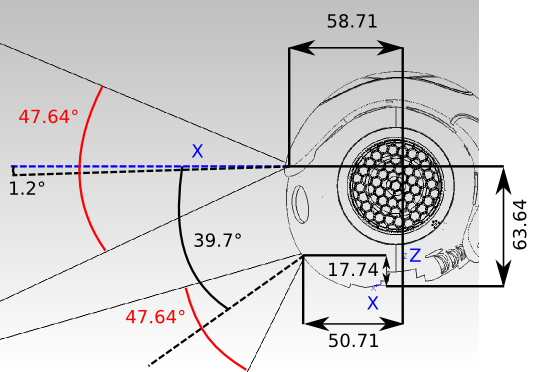
\includegraphics[height=5cm]{figures/nao_camera_lateral.png} 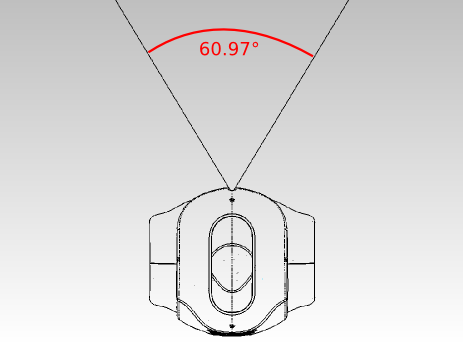
\includegraphics[height=5cm]{figures/nao_camera_top.png} 

	





\chapter{Zielsetzung}
Im Rahmen ... (Was will ich ueberhaupt mit meiner Abreit erreichen? Etwas verbessern, entwickeln, vergleichen...)


\chapter{Aufgabenpakete}
Ausgehend von der Zielbeschreibung werden folgende Arbeitspakete definiert:

\begin{itemize}
	\item Einarbeitung in das Themenbereich. Dazu geh�rt die Evaluierung relevanter Paper sowie das Ber�cksichtigen der bereits verf�gbaren Komponenten und Implemaentationen. Das Arbeitsergebnis ist eine Zusammenfassung relevanter Arbeiten.

	\item Entwicklung eines Ansatzes ...

	\item Analyse, Design und Entwurf einer Architektur

	\item Definition von geeigneten Testszenarien

	\item Umsetzung der Architektur, Implementierung

	\item Dokumentation der Architektur und des Programmcodes
\end{itemize}

	
\chapter{Zeitplan}
Die Bearbeitung dauert maximal 6 Monate. (Am besten eignet sich ein Gannt Diagramm)

\chapter{Organisatorisches}
\begin{itemize}
	\item Sprache der Diplomarbeit:
	\item Textverarbeitungssystem:
	\item Programmiersprache: Java 1.5
	\item Betreuer: 
	\item Gutachter: Prof. Dr. Sahin Albayrak, Dr.- Ing. Stefan Fricke
\end{itemize}

\chapter{Anhang}



